\begin{table}[H]\centering\small

\begin{tabular}{lrrrrrr}

\toprule

& \multicolumn{3}{c}{Null rejection (\%)} & \multicolumn{3}{c}{Design power (\%)} \\

Rule & 400 & 800 & 1600 & 400 & 800 & 1600 \\

\midrule

Past-mean certificate & 0.11 & 0.22 & 0.32 & 11.41 & 37.76 & 78.29 \\

Fixed certificate & 0.02 & 0.19 & 0.96 & 4.00 & 44.94 & 93.04 \\

Fixed log growth & 0.69 & 1.44 & 1.98 & 28.31 & 66.50 & 92.44 \\

One-block power & 1.20 & 1.36 & 1.36 & 25.53 & 34.10 & 36.04 \\

Horizon DP & 1.42 & 1.84 & 2.25 & 37.48 & 72.83 & 97.07 \\

Refined horizon DP & 1.41 & 1.83 & 2.26 & 37.47 & 72.81 & 97.13 \\

\bottomrule\end{tabular}

\caption{Review-time rejection fractions from 20,000 paths per law. The null has mean zero and the design alternative mean .1, both with variance one. Every rule has the same individual nominal 5\% bound, public moment cap and bet/review calendar; observed null rates differ. Each horizon-DP entry uses a separate policy targeting that deadline.}\label{tab:lambda-power}\end{table}

At 400 observations the horizon rule crosses on 7496/20000 paths (37.48\%) versus 2281/20000 (11.41\%) for the past-mean rule. The paired difference is 26.08 percentage points (Monte Carlo 95\% interval [25.47, 26.68]). This compares a common nominal level, not matched actual null-crossing probabilities. At the longest deadline the fixed log-growth rule does not outperform the fixed certificate rule, illustrating that the objectives differ. The repeatedly greedy one-block rule also falls short of the deadline-specific policy.

The refined-grid powers closely agree with the primary implementation, and all six predicted-versus-observed design-power checks pass the declared numerical-plus-Monte-Carlo audit. All pre-block horizon-policy and fixed stakes, every first crossing, and the complete summary are independently reconstructed (12,331,336 scalar checks). Direct multiplicative score replay covers the first sixteen paths under each law; it is not a replay of every score path. Its maximum log-capital discrepancy is 6.17e-14. The stronger alternatives .2 and .3 are retained in the numeric report. No result supplies a power optimum for a changing financial score law or improved fund performance.

\begin{figure}[H]\centering

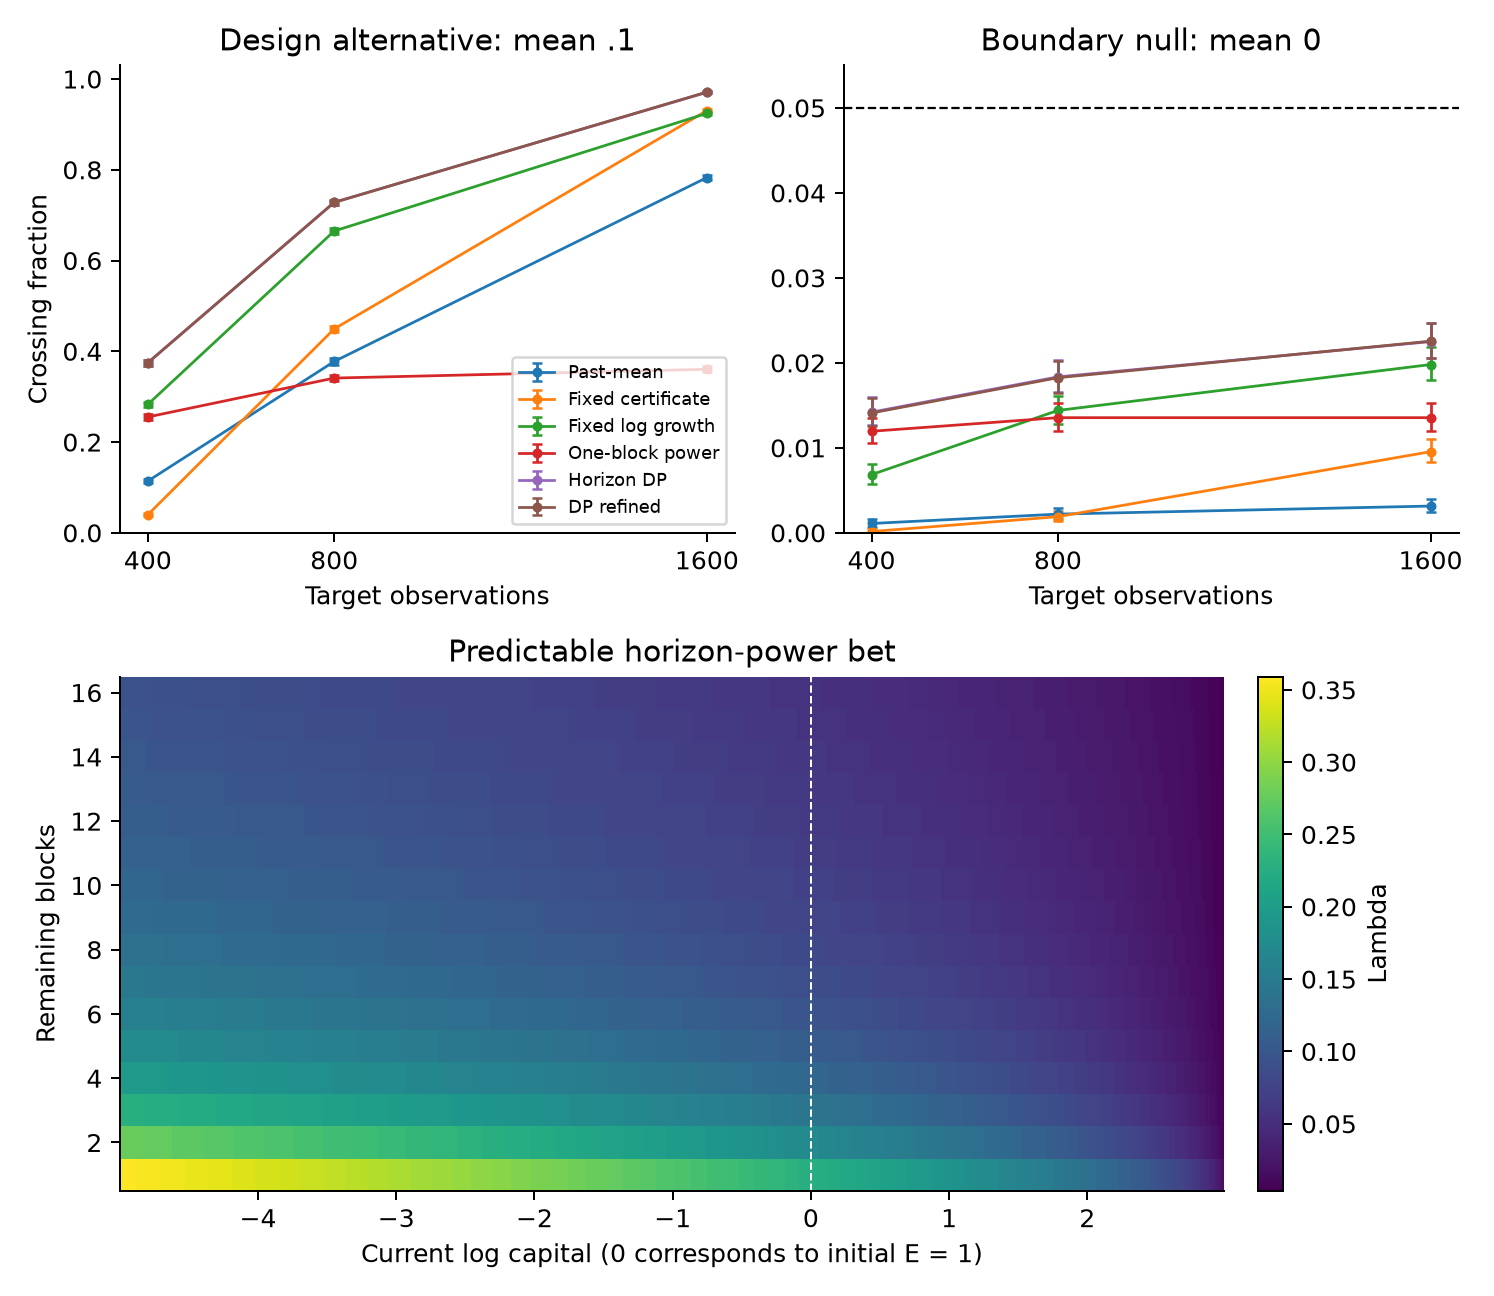
\includegraphics[width=.97\linewidth]{figures/lambda_power.png}

\caption{Top: observed design-power and null-crossing fractions with pointwise Wilson 95\% intervals. Each DP point uses its own target horizon; the connected points are not one policy monitored at three dates. Bottom: the primary working-model bet as a function of pre-block log capital and remaining blocks. Bets and decisions share the 100-observation calendar.}\label{fig:lambda-power}\end{figure}
